%! Author = admin
%! Date = 07.12.2022

% Preamble
\documentclass[a4paper,12pt]{article}

% Packages
\usepackage{multirow}
\usepackage{wrapfig}
\usepackage[T2A]{fontenc}
\usepackage[utf8]{inputenc}
\usepackage[english,russian]{babel}
\usepackage{indentfirst}
\usepackage[usenames]{color}
\usepackage[a4paper,top=0.75cm,bottom=0.75cm,left=0.75cm,right=0.75cm,marginparwidth=0.75cm]{geometry}
\usepackage{colortbl}
\usepackage{graphicx}%Вставка картинок правильная
\usepackage{float}%"Плавающие" картинки
\usepackage{wrapfig}
\usepackage{hyperref}
\usepackage{subcaption}
\usepackage[rgb]{xcolor}
\usepackage{todonotes}
\usepackage{amsmath,amsfonts,amssymb,amsthm,mathtools}
\usepackage{makecell}


% package to open file containing variables
\usepackage{datatool, filecontents}
\usepackage{colortbl}
\usepackage{booktabs}
\DTLsetseparator{,}% Set the separator between the columns.

% import data
\DTLloadrawdb[noheader, keys={thekey,thevalue}]{output_data}{C:/labas/1.2.4/data/output_data.csv}
% Loads output_data.csv with column headers 'thekey' and 'thevalue'
\newcommand{\var}[1]{\DTLfetch{output_data}{thekey}{#1}{thevalue}}

% Document
\begin{document}

    \begin{centering}
        \section* {{\fboxsep=0pt\colorbox{green!50}{\strut Обработка данных:}}}
    \end{centering}

    \subsection* {Размеры тел}

    \begin{table}[h!]
        \centering
        \begin{tabular}{|c|c|c|c|c|c|c|c|c|}
            \hline
            & $a_{\text{к}}$ & $a$ & $b$ & $c$ & $h_{\text{ц}}$ & $r_{\text{ц}}$ & $h_{\text{д}}$ & $r_{\text{д}}$
            \\ \hline
            значение, см & \var{ak} & \var{a} & \var{b} & \var{c} & \var{hc} & \var{rc} & \var{hd} & \var{rd}
            \\ \hline
            $\varepsilon$ & \var{reak} & \var{rea} & \var{reb} & \var{rec} & \var{rehc} & \var{rerc} & \var{rehd} & \var{rerd}
            \\ \hline
        \end{tabular}
        \caption{Размеры исследуемых тел и их погрешности}
    \end{table}

    Абсолютная погрешность измерения размеров линейкой составляет 0.005 см.

    \subsection*{Периоды колебаний}

    \begin{table}[h!]
        \centering
        \begin{tabular}{|c|c|c|c|c|c|c|c|c|c|c|}
            \hline
            $T$ & $T_{\text{1z}}$ & $T_{\text{1x}}$ & $T_{\text{1y}}$ & $T_{\text{1d}}$ & $T_{\text{1e}}$ & $T_{\text{1p}}$ & $T_{\text{1m}}$ & $T_{\text{2x}}$ & $T_{\text{2y}}$ & $T_{\text{2z}}$
            \\ \hline
            $T_{\text{cp}}$, c & \var{T1z} & \var{T1x} & \var{T1y} & \var{T1d} & \var{T1e} & \var{T1p} & \var{T1m} & \var{T2x} & \var{T2y} & \var{T2z}
            \\ \hline
            $\sigma_{\text{случ}}$, c & \var{rdeT1z} & \var{rdeT1x} & \var{rdeT1y} & \var{rdeT1d} & \var{rdeT1e} & \var{rdeT1p} & \var{rdeT1m} & \var{rdeT2x} & \var{rdeT2y} & \var{rdeT2z}
            \\ \hline
            $\sigma_{\text{полн}}$, c & \var{feT1z} & \var{feT1x} & \var{feT1y} & \var{feT1d} & \var{feT1e} & \var{feT1p} & \var{feT1m} & \var{feT2x} & \var{feT2y} & \var{feT2z}
            \\ \hline
            $\varepsilon_{\text{полн}}$ & \var{reT1z} & \var{reT1x} & \var{reT1y} & \var{reT1d} & \var{reT1e} & \var{reT1p} & \var{reT1m} & \var{reT2x} & \var{reT2y} & \var{reT2z}
            \\ \hline
        \end{tabular}


        \begin{tabular}{|c|c|c|c|c|c|c|c|c|c|}
            \hline
            $T$ & $T_{\text{2d}}$ & $T_{\text{2e}}$ & $T_{\text{2m}}$ & $T_{\text{2p}}$ & $T_{\text{p}}$ & $T_{\text{3x}}$ & $T_{\text{3y}}$ & $T_{\text{4x}}$ & $T_{\text{4y}}$
            \\ \hline
            $T_{\text{cp}}$, c & \var{T2d} & \var{T2e} & \var{T2m} & \var{T2p} & \var{Tp} & \var{T3x} & \var{T3y} & \var{T4x} & \var{T4y}
            \\ \hline
            $\sigma_{\text{случ}}$, c & \var{rdeT2d} & \var{rdeT2e} & \var{rdeT2m} & \var{rdeT2p} & \var{rdeTp} & \var{rdeT3x} & \var{rdeT3y} & \var{rdeT4x} & \var{rdeT4y}
            \\ \hline
            $\sigma_{\text{полн}}$, c & \var{feT2d} & \var{feT2e} & \var{feT2m} & \var{feT2p} & \var{feTp} & \var{feT3x} & \var{feT3y} & \var{feT4x} & \var{feT4y}
            \\ \hline
            $\varepsilon_{\text{полн}}$ & \var{reT2d} & \var{reT2e} & \var{reT2m} & \var{reT2p} & \var{reTp} & \var{reT3x} & \var{reT3y} & \var{reT4x} & \var{reT4y}
            \\ \hline
        \end{tabular}
        \caption{Средние значения периодов колебаний ($T_{\text{cp}}$) и их погрешности}
        \label{periods}
    \end{table}

    Систематическая погрешность для всех измерений одинакова и складывается из погрешности секундомера и скорости
    реакции экспериментатора, которая определяется с помощью измерения временного промежутка между двумя нажатиями
    на кнопку. В моем случае скорость реакции составляет 0.13 с, а погрешность секундомера - 0.001 с, следовательно
    ей можно пренебречь и принять систематическую погрешность равной 0.13 с.

    \subsection* {Проверка соотношений периодов}

    \begin{itemize}
        \item {Параллелепипед}

        $$\frac{a^2 T_{\text{2x}}^2 + b^2 T_{\text{2y}}^2 + c^2 T_{\text{2z}}^2}{a^2 + b^2 +c^2} = T_{\text{2d}}^2, \quad
        \frac{a^2 T_{\text{2x}}^2 + b^2 T_{\text{2y}}^2 + c^2 T_{\text{2z}}^2}{a^2 + b^2 +c^2} =
        (\var{form21} \pm \var{error21}) c^2, \quad
        T_{\text{2d}}^2 = (\var{T2d**2} \pm 0.26) c^2 $$

        $$\frac{b^2 T_{\text{2y}}^2 + c^2 T_{\text{2z}}^2}{c^2 + b^2} = T_{\text{2e}}^2, \quad
        \frac{b^2 T_{\text{2y}}^2 + c^2 T_{\text{2z}}^2}{c^2 + b^2} = (\var{form22} \pm \var{error22}) c^2, \quad
        T_{\text{2e}}^2 = (\var{T2e**2} \pm 0.26) c^2$$

        $$\frac{a^2 T_{\text{2x}}^2 + c^2 T_{\text{2z}}^2}{c^2 + a^2} = T_{\text{2p}}^2, \quad
        \frac{a^2 T_{\text{2x}}^2 + c^2 T_{\text{2z}}^2}{c^2 + a^2} = (\var{form23} \pm \var{error23}) c^2, \quad
        T_{\text{2p}}^2 = (\var{T2p**2} \pm 0.26) c^2$$

        $$\frac{b^2 T_{\text{2y}}^2 + a^2 T_{\text{2x}}^2}{a^2 + b^2} = T_{\text{2m}}^2, \quad
        \frac{b^2 T_{\text{2y}}^2 + a^2 T_{\text{2x}}^2}{a^2 + b^2} = (\var{form24} \pm \var{error24}) c^2, \quad
        T_{\text{2m}}^2 = (\var{T2m**2} \pm 0.262) c^2$$

        \item {Куб}

        В справедливости соотношения:
        $T_{\text{1z}} = T_{\text{1x}} = T_{\text{1y}} = T_{\text{1d}} = T_{\text{1e}} = T_{\text{1p}} = T_{\text{1m}}$
        можно убедиться, исходя из тaблицы \ref{periods}.

        $$\frac{T_{\text{1x}}^2 + T_{\text{1y}}^2 + T_{\text{1z}}^2}{3} = T_{\text{1d}}^2, \quad
        \frac{T_{\text{1x}}^2 + T_{\text{1y}}^2 + T_{\text{1z}}^2}{3} = (\var{form11} \pm \var{error11}) c^2, \quad
        T_{\text{1d}}^2 = (\var{T1d**2} \pm 0.26) c^2$$

        $$\frac{T_{\text{1y}}^2 + T_{\text{1z}}^2}{2} = T_{\text{1e}}^2, \quad
        \frac{T_{\text{1y}}^2 + T_{\text{1z}}^2}{2} = (\var{form12} \pm \var{error12}) c^2, \quad
        T_{\text{1e}}^2 = (\var{T1e**2} \pm 0.26) c^2$$

        $$\frac{T_{\text{1x}}^2 + T_{\text{1z}}^2}{2} = T_{\text{1p}}^2, \quad
        \frac{T_{\text{1x}}^2 + T_{\text{1z}}^2}{2} = (\var{form13} \pm \var{error13}) c^2, \quad
        T_{\text{1p}}^2 = (\var{T1p**2} \pm 0.26) c^2$$

        $$\frac{T_{\text{1y}}^2 + T_{\text{1x}}^2}{2} = T_{\text{1m}}^2, \quad
        \frac{T_{\text{1y}}^2 + T_{\text{1x}}^2}{2} = (\var{form14} \pm \var{error14}) c^2, \quad
        T_{\text{1m}}^2 = (\var{T1m**2} \pm 0.26) c^2$$


        \item {Цилиндр}

        $$\frac{T_{\text{3y}}^2}{T_{\text{3x}}^2} = 1 + \frac{h_{\text{ц}}^2}{3 r_{\text{ц}}^2}, \quad
        \frac{T_{\text{3y}}^2}{T_{\text{3x}}^2} = (\var{form32} \pm \var{error32}), \quad
        1 + \frac{h_{\text{ц}}^2}{3 r_{\text{ц}}^2} = (\var{form31} \pm \var{error31})$$


        \item {Диск}

        $$\frac{T_{\text{4y}}^2}{T_{\text{4x}}^2} = 1 + \frac{h_{\text{д}}^2}{3 r_{\text{д}}^2}, \quad
        \frac{T_{\text{4y}}^2}{T_{\text{4x}}^2} = (\var{form42} \pm \var{error42}), \quad
        1 + \frac{h_{\text{д}}^2}{3 r_{\text{д}}^2} = (\var{form41} \pm \var{error41})$$

    \end{itemize}

    \subsection* {Эллипсоиды инерции}

    Поскольку мы не знаем сами моменты инерции, но знаем их соотношения и пропорциональность квадратам периодов,
    построим сечения эллипсоидов в произвольном масштабе, согласно уравнению эллипсоида:

    $$\frac{x^2}{A^2} + \frac{y^2}{B^2} + \frac{z^2}{C^2} = 1$$

    \begin{itemize}

        \item{Параллелепипед}

        $$A = \frac{1}{\sqrt{T_{\text{2x}}^2 - T_{\text{p}}^2}} = \var{ax2x}, \qquad
        B = \frac{1}{\sqrt{T_{\text{2y}}^2 - T_{\text{p}}^2}} = \var{ax2y}, \qquad
        C = \frac{1}{\sqrt{T_{\text{2z}}^2 - T_{\text{p}}^2}} = \var{ax2z}$$


        \begin{figure}[h!!]

            \begin{subfigure}{0.33\textwidth}
                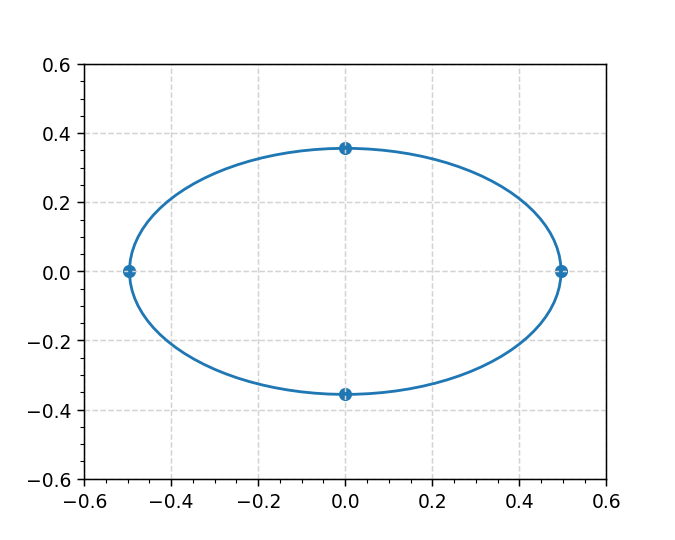
\includegraphics[width=\linewidth, height=\linewidth]{par_xz.png}
                \caption*{Сечение плоскостью xz}
                \label{fig:subim1}
            \end{subfigure}
            \begin{subfigure}{0.33\textwidth}
                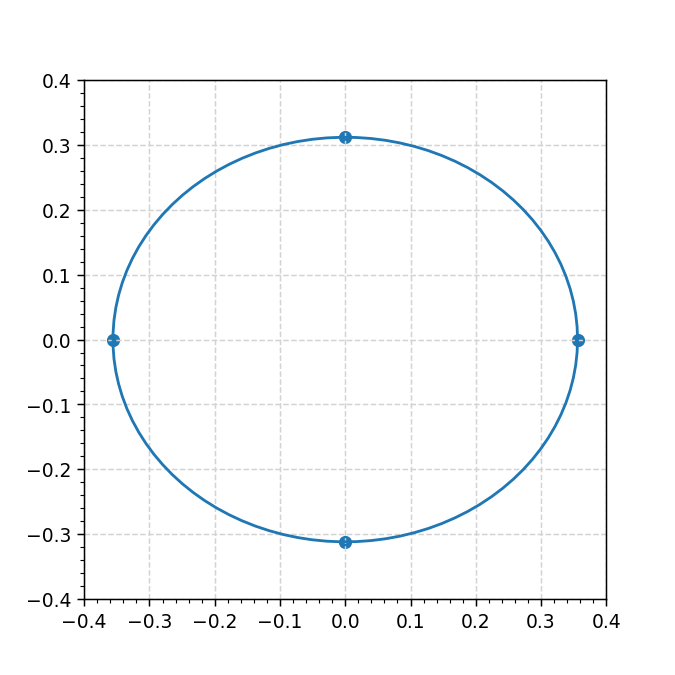
\includegraphics[width=\linewidth, height=\linewidth]{par_xy.png}
                \caption*{Сечение плоскостью xy}
                \label{fig:subim2}
            \end{subfigure}
            \begin{subfigure}{0.33\textwidth}
                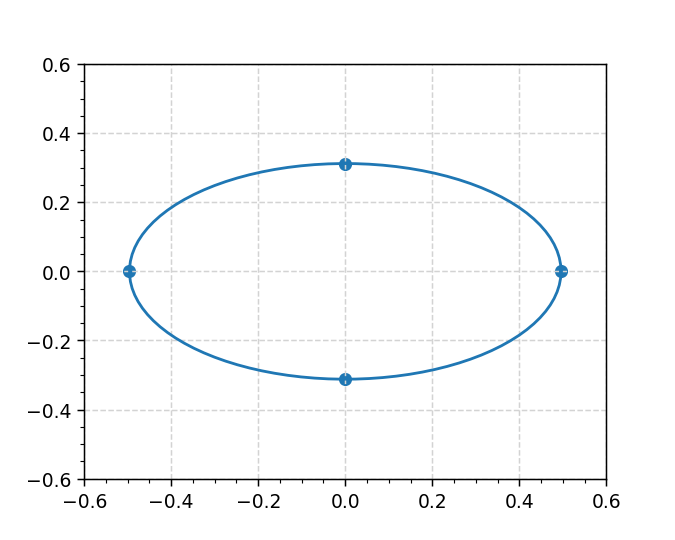
\includegraphics[width=\linewidth, height=\linewidth]{par_yz.png}
                \caption*{Сечение плоскостью yz}
                \label{fig:subim3}
            \end{subfigure}

        \end{figure}


    \end{itemize}


\end{document}
